% Nallino, Part I p. 306: the sextile ray of a planet R with latitude RS: the arc RS perpendicular to the
% ecliptic, the ray RA and the dotted circle about R through A, touching the ecliptic at S, redrawn from the print.
% Measured on the scan (_intake/latin/tools/fig306).
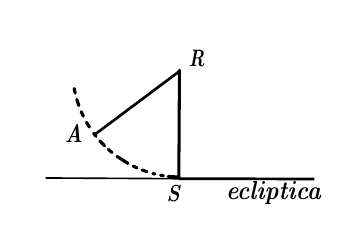
\begin{tikzpicture}[x=0.9907pt,y=-0.9907pt,line cap=butt,every node/.style={font=\fontsize{11}{11}\bfseries\itshape\selectfont,inner sep=0pt}]
\useasboundingbox (0,0) rectangle (108.00,66.00);
\draw[line width=1.10pt] (55.36,15.47) -- (55.13,55.09);  % the arc RS, from its round top at R to the ecliptic at S
\draw[line width=0.96pt] (24.44,39.00) -- (55.36,15.89);  % the ray RA, from the dotted circle at A to R
\draw[line width=0.98pt] (55.13,55.09) -- (104.61,55.18);  % the ecliptic right of S
\draw[line width=0.59pt] (6.51,54.82) -- (55.13,55.09);  % the ecliptic left of S, thinner as printed
\fill (55.36,15.47) circle[radius=0.55];  % the round top of RS at R
% the dotted circle about R through A, dash by dash
\draw[line width=1.14pt,line cap=round] (55.26,54.51)--(51.27,54.25) (49.49,54.00)--(48.49,53.83) (46.39,53.37)--(45.68,53.19) (43.49,52.54)--(41.74,51.92) (39.85,51.14)--(38.50,50.51) (36.60,49.52)--(32.60,46.97) (30.75,45.54)--(29.43,44.40) (27.99,43.04)--(26.32,41.28);
\draw[line width=1.14pt,line cap=round] (24.93,39.63)--(24.05,38.48) (22.52,36.26)--(21.45,34.49) (20.31,32.31)--(19.54,30.65) (18.64,28.38)--(17.92,26.16) (17.32,23.88)--(16.97,22.20);
\node at (61.67,11.31) {\normalfont\fontsize{11}{11}\bfseries\itshape\selectfont \resizebox{5.66pt}{5.89pt}{R}};
\node at (16.79,38.85) {\normalfont\fontsize{11}{11}\bfseries\itshape\selectfont \resizebox{6.44pt}{6.28pt}{A}};
\node at (53.11,60.45) {\normalfont\fontsize{11}{11}\bfseries\itshape\selectfont \resizebox{4.80pt}{5.74pt}{S}};
\node at (89.60,60.42) {\normalfont\fontsize{11}{11}\bfseries\itshape\selectfont \resizebox{34.20pt}{6.54pt}{ecliptica}};
\end{tikzpicture}
